\chapter{Evaluación experimental: tablas completas}
\label{apendice:evaluacion}

Este anexo recoge el detalle por caso de los experimentos del capítulo~\ref{cap:evaluacion} que en el cuerpo se resumen con medianas o con una figura, más las figuras secundarias del estudio de formatos y la lista de casos de los bancos. Todo se regenera desde el repositorio: cada experimento tiene su documento, sus resultados crudos en JSON y el script que produce tablas y figuras, en la carpeta \texttt{feedback-docs} del repositorio (subcarpetas \texttt{experimentos-motor}, \texttt{experimentos-objetivo}, \texttt{estudio-formatos} y \texttt{auditoria-planes-8e}), con los harness en \texttt{backend/scripts}.

\section{Casos de los bancos}
\label{sec:anexoCasosBancos}

El banco del solver tiene ocho casos con veredicto esperado:

\begin{enumerate}
\item María, 3 días y 3 comidas, sin restricciones configurables. Factible.
\item María, 7 días y 5 comidas, objetivo calórico blando de $1\,500$ kcal. Factible; cada día dentro de $\pm 50$ kcal y la media dentro de $\pm 25$.
\item María, 7 días y 5 comidas, objetivo calórico y preferencia vegetariana. Factible, con predominio vegetariano y el mismo criterio de bandas.
\item John, 7 días y 5 comidas, alergia al cacahuete dura y mínimo de proteína blando. Factible.
\item Emma, 7 días y 5 comidas, intolerancia a la lactosa dura y máximo de sodio blando. Factible.
\item John, 3 días y 5 comidas, 900 kcal duras y 180 g de proteína duros. Infactible, con las dos filas en el núcleo de conflicto.
\item Mínimo de proteína de 200 g duro con casi todas las fuentes prohibidas, construido contra el catálogo real. Infactible.
\item Diseño: ejercita la no repetición por etiqueta, el tope de raciones por periodo, el reparto por comidas y la preferencia por alimento. Factible.
\end{enumerate}

Sobre esos casos el banco comprueba además las garantías de las reglas base y de la plausibilidad (tope de apariciones por día, variedad mínima, raciones dentro del perfil de cada alimento, franjas, roles de condimento y dulce), hasta las 32 comprobaciones de la tabla~\ref{tab:bancos}.

La prueba de extremo a extremo contra el backend desplegado corre doce casos por la API, los seis primeros anclados a clientes reales con sus restricciones de la base de datos y los otros seis con perfiles sintéticos:

\begin{enumerate}
\item María, 3 días, sin restricciones. Factible.
\item María, 7 días, objetivo calórico blando. Factible, desviación menor del 5\,\%.
\item María, 7 días, objetivo calórico y preferencia vegetariana. Factible, predominio vegetariano.
\item John, 7 días, alergia dura y mínimo de proteína. Factible.
\item Emma, 7 días, intolerancia dura y máximo de sodio. Factible.
\item John, 3 días, 900 kcal duras y 180 g de proteína duros. Infactible.
\item Sintético, 7 días y 4 comidas, objetivo calórico y reparto por comidas. Factible.
\item Sintético, 7 días y 5 comidas, carne roja como mucho dos veces por semana, duro. Factible.
\item Sintético, 7 días y 3 comidas, no repetir un alimento en 4 días, blando. Factible.
\item Sintético, 7 días y 3 comidas, no repetir pescado en 2 días, blando. Factible.
\item Estilo del profesional por ámbito nutricionista. Factible y refleja el estilo.
\item Sintético, 7 días y 5 comidas, mínimo alto de calcio con las familias ricas en calcio prohibidas. Infactible.
\end{enumerate}

A los doce se suman el flujo de firma de un plan y el rechazo de una petición sin token, hasta las 29 comprobaciones.

\section{Magnitudes de la función objetivo por caso}
\label{sec:anexoMagnitudes}

Contribución ponderada realizada de cada familia del objetivo, en unidades del objetivo, antes del ajuste de pesos (sección~\ref{sec:evalMagnitudes}). Un guion indica que el caso no lleva ese término.

\begin{table}[htbp]
\centering
\scriptsize
\setlength{\tabcolsep}{4pt}
\begin{tabular}{|l|r|r|r|r|r|r|r|}
\hline
\textbf{Caso} & \textbf{kcal} & \textbf{macro} & \textbf{nutriente} & \textbf{reparto comidas} & \textbf{prefer.} & \textbf{variedad} & \textbf{reparto plan} \\
\hline
banco 2 & 0 & -- & -- & -- & -- & 0 & 0 \\
\hline
banco 3 & 0 & -- & -- & -- & $2\,224$ & 100 & 0 \\
\hline
banco 4 & -- & -- & 0 & -- & -- & 35 & 4 \\
\hline
banco 5 & -- & -- & 0 & -- & -- & 60 & 0 \\
\hline
banco 8 & -- & -- & -- & $33\,036\,100\,000$ & 96 & 195 & 4 \\
\hline
David & $119\,000$ & -- & -- & -- & -- & 215 & 4 \\
\hline
Lucía & -- & -- & 0 & -- & $2\,688$ & 230 & 0 \\
\hline
Sofía & -- & -- & 0 & -- & -- & 45 & 0 \\
\hline
Tomás & $694\,932\,000$ & $4\,899\,720$ & -- & $62\,508\,450\,000$ & -- & 135 & 0 \\
\hline
Carlos & $51\,100$ & -- & -- & -- & -- & 220 & 0 \\
\hline
Nadia & -- & -- & -- & -- & $2\,688$ & 60 & 0 \\
\hline
\end{tabular}
\caption{Contribución de cada familia al objetivo, por caso, antes del ajuste. El término de preferencias es negativo en el objetivo (premia), y aquí se da en valor absoluto.}
\label{tab:anexoContribuciones}
\end{table}

Cociente $Q$ por caso y familia, antes del ajuste (rango completo alcanzable de la familia dividido por el coste de una unidad natural de desviación del término nutricional dominante):

\begin{table}[htbp]
\centering
\small
\begin{tabular}{|l|c|c|c|}
\hline
\textbf{Caso} & \textbf{Preferencias} & \textbf{Reparto del plan} & \textbf{Variedad} \\
\hline
banco 2 & -- & 0,0514 & 0,0071 \\
\hline
banco 3 & 0,0320 & 0,0514 & 0,0071 \\
\hline
banco 4 & -- & 0,0750 & 0,0104 \\
\hline
banco 5 & -- & 0,0514 & 0,0071 \\
\hline
banco 8 & 0,0000 & 0,0001 & 0,0000 \\
\hline
David & -- & 0,0514 & 0,0071 \\
\hline
Lucía & 0,0560 & 0,0750 & 0,0104 \\
\hline
Sofía & -- & 0,0900 & 0,0125 \\
\hline
Tomás & -- & 0,0001 & 0,0000 \\
\hline
Carlos & -- & 0,0514 & 0,0071 \\
\hline
mediana & 0,0320 & 0,0514 & 0,0071 \\
\hline
\end{tabular}
\caption{$Q$ por caso antes del ajuste de pesos. Tras multiplicar por $1\,000$ los pesos no nutricionales, cada valor se multiplica por $1\,000$ (medianas 32, 51 y 7).}
\label{tab:anexoQ}
\end{table}

\section{Rotura de simetría: valores por caso}
\label{sec:anexoSimetria}

Detalle de la sección~\ref{sec:evalSimetria}: estado, tiempo medio y objetivo (menor es mejor) en cada brazo, con 5 repeticiones por caso.

\begin{table}[htbp]
\centering
\small
\begin{tabular}{|p{1.4cm}|p{4.2cm}|p{7.4cm}|}
\hline
\textbf{Caso} & \textbf{Sin rotura} & \textbf{Cadena lexicográfica} \\
\hline
banco 2 & óptimo, 4,9 s & óptimo, 5,2 s \\
\hline
banco 3 & óptimo, 22,4 s & óptimo, 23,3 s \\
\hline
banco 4 & óptimo, 69,7 s & 5 de 5 en el límite; objetivo de $5\,000$ a $14\,000$ \\
\hline
banco 5 & óptimo, 66,7 s & 5 de 5 en el límite; objetivo de $60\,000$ a $85\,000$ \\
\hline
David & límite, desviación 0,02\,\% & límite, desviación 0,56\,\%; objetivo 13 veces peor \\
\hline
Lucía & límite & límite, objetivo algo peor \\
\hline
Sofía & límite sin óptimo & 3 de 5 óptimos a 79,7 s; objetivo de $110\,000$ a $45\,000$ \\
\hline
Tomás & óptimo, 9,8 s & óptimo, 11,2 s \\
\hline
Carlos & límite & límite, objetivo de $495\,300$ a $338\,400$ \\
\hline
Nadia & óptimo, 52,9 s & 3 de 5 sin probar óptimo, 85,6 s \\
\hline
\end{tabular}
\caption{Cadena lexicográfica frente al motor sin rotura.}
\label{tab:anexoSimetriaLex}
\end{table}

\begin{table}[htbp]
\centering
\small
\begin{tabular}{|p{1.4cm}|p{5.2cm}|p{6.4cm}|}
\hline
\textbf{Caso} & \textbf{Sin orden} & \textbf{Orden escalar (energía diaria no creciente)} \\
\hline
banco 2 & óptimo, 4,9 s & óptimo, 3,2 s \\
\hline
banco 3 & óptimo, 22,4 s & óptimo, 9,7 s \\
\hline
banco 4 & óptimo, 69,7 s; objetivo $5\,000$ & 5 de 5 en el límite; objetivo $100\,000$ \\
\hline
banco 5 & óptimo, 66,7 s; objetivo $60\,000$ & 5 de 5 en el límite; objetivo $75\,000$ \\
\hline
David & límite; objetivo $430\,100$ & límite; objetivo $230\,100$ \\
\hline
Lucía & límite; objetivo $-2\,414\,000$ & límite; objetivo $-2\,453\,000$ \\
\hline
Sofía & 80,8 s, 1 de 5 óptimos & 63,5 s, 5 de 5 óptimos; objetivo de $110\,000$ a $45\,000$ \\
\hline
Tomás & óptimo, 9,8 s & óptimo, 15,3 s \\
\hline
Carlos & límite; objetivo $495\,300$ & límite; objetivo $387\,200$ \\
\hline
Nadia & óptimo, 52,9 s & óptimo, 69,8 s \\
\hline
\end{tabular}
\caption{Variante escalar frente al motor sin orden.}
\label{tab:anexoSimetriaEscalar}
\end{table}

\section{Bandas de tolerancia: desviaciones con signo}
\label{sec:anexoBandas}

Para cada caso afectado de la sección~\ref{sec:evalBandas}: media con signo del plan en las tres repeticiones, peor día y exceso fuera de la banda diaria y de la banda de la media.

\begin{table}[htbp]
\centering
\small
\begin{tabular}{|p{2.7cm}|p{1.2cm}|p{4cm}|p{1.7cm}|p{2.2cm}|}
\hline
\textbf{Caso} & \textbf{Brazo} & \textbf{Media con signo (kcal)} & \textbf{Peor día (kcal)} & \textbf{Fuera de banda} \\
\hline
banco 2 & base & 0,0 / 0,0 / 0,0 & 0,0 & 0 / 0 \\
\hline
banco 2 & A y B & $-20{,}7$ en las tres & 49,9 & 0 / 0 \\
\hline
banco 3 & base & 0,0 / 0,0 / 0,0 & 0,0 & 0 / 0 \\
\hline
banco 3 & A & $-23{,}1$ / $-21{,}4$ / $-3{,}0$ & 50,0 & 0 / 0 \\
\hline
banco 3 & B & $-16{,}4$ / $+21{,}5$ / $+24{,}7$ & 49,9 & 0 / 0 \\
\hline
David & base & $-0{,}2$ en las tres & 0,5 & 0 / 0 \\
\hline
David & A & $-5{,}0$ en las tres & 28,0 & 0 / 0 \\
\hline
David & B & $-11{,}8$ en las tres & 49,1 & 0 / 0 \\
\hline
Carlos & base & $-0{,}2$ en las tres & 0,6 & 0 / 0 \\
\hline
Carlos & A & $-5{,}5$ en las tres & 40,7 & 0 / 0 \\
\hline
Carlos & B & $-0{,}3$ en las tres & 0,9 & 0 / 0 \\
\hline
diseño macro (kcal) & A & $+24{,}5$ / $-21{,}3$ / $-5{,}1$ & 49,9 & 0 / 0 \\
\hline
diseño macro (kcal) & B & $+12{,}2$ / 0,0 / $-21{,}3$ & 50,0 & 0 / 0 \\
\hline
diseño macro (proteína, g) & A & $+0{,}9$ / $+1{,}4$ / $+1{,}7$ & 4,5 & 0 / 0 \\
\hline
diseño macro (proteína, g) & B & $+1{,}9$ / $+0{,}8$ / $+1{,}4$ & 4,5 & 0 / 0 \\
\hline
\end{tabular}
\caption{Desviaciones del objetivo por caso afectado, brazo y repetición. La última columna es el exceso fuera de la banda diaria y fuera de la banda de la media.}
\label{tab:anexoBandasDesv}
\end{table}

\begin{figure}[htbp]
\begin{center}
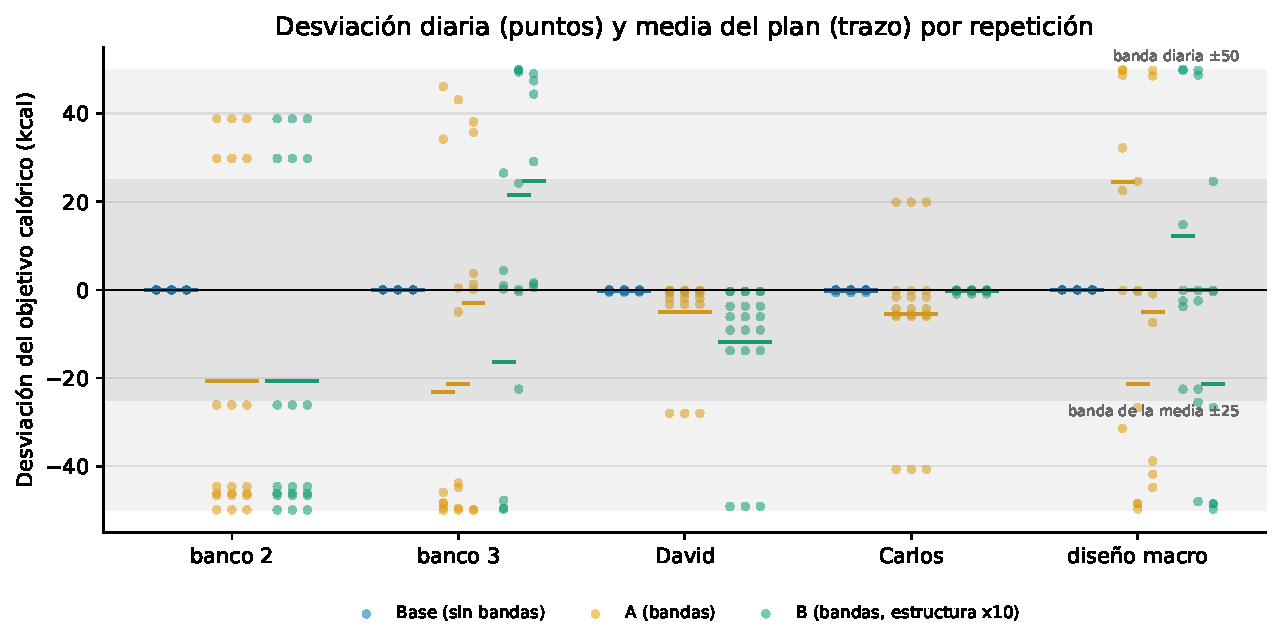
\includegraphics[width=0.95\textwidth]{Imagenes/Vectorial/fig_bandas_desviacion}
\end{center}
\caption{Desviación diaria (puntos) y media del plan (trazo) por repetición en los casos afectados limpios. Las franjas grises son la banda diaria de $\pm 50$ kcal y la banda de la media de $\pm 25$. Tomás, el caso de conflicto, queda fuera de la figura porque su desviación de $-1\,240$ kcal aplastaría la escala.}
\label{fig:anexoBandasDesv}
\end{figure}

\section{Estudio de formatos: detalle}
\label{sec:anexoFormatos}

Los cinco formatos del estudio de la sección~\ref{sec:evalFormatos}, con el mismo mensaje redactado en cada uno:

\begin{table}[htbp]
\centering
\small
\begin{tabular}{|l|p{4cm}|p{7cm}|}
\hline
\textbf{Formato} & \textbf{Descripción} & \textbf{Mensaje 2} \\
\hline
Natural & texto libre de un nutricionista, línea base & Busca ganar músculo, es alérgico al cacahuete y quiero al menos 140 g de proteína al día. \\
\hline
Telegráfico & lista de viñetas & - alergia: cacahuete / - proteína: mínimo 140 g/día / - objetivo: ganar músculo \\
\hline
Plantilla & campos con etiqueta legible & Objetivo: ganar músculo. Evitar: cacahuete (alergia). Mínimos: 140 g de proteína al día. \\
\hline
Clave-valor & pares casi de configuración & alergia=cacahuete; proteina\_min=140g/dia; objetivo=ganar\_musculo \\
\hline
Verboso & conversacional con contexto irrelevante de consulta & Este chico entrena fuerza cuatro días a la semana y me pregunta mucho por los batidos... quiero que llegue al menos a 140 g de proteína al día, y mucho cuidado porque es alérgico al cacahuete. \\
\hline
\end{tabular}
\caption{Los cinco formatos del estudio sobre el mismo mensaje.}
\label{tab:anexoFormatos}
\end{table}

\begin{table}[htbp]
\centering
\small
\begin{tabular}{|l|c|c|c|}
\hline
\textbf{Formato} & \textbf{Latencia media} & \textbf{Tokens de entrada} & \textbf{Tokens de salida} \\
\hline
Natural & 20,4 s (d.t. 8,8) & $1\,555$ & 67 \\
\hline
Telegráfico & 20,5 s (d.t. 4,3) & $1\,550$ & 63 \\
\hline
Plantilla & 17,5 s (d.t. 3,8) & $1\,555$ & 63 \\
\hline
Clave-valor & 15,9 s (d.t. 2,7) & $1\,547$ & 64 \\
\hline
Verboso & 16,0 s (d.t. 2,5) & $1\,588$ & 64 \\
\hline
\end{tabular}
\caption{Latencia y tokens por llamada al traductor, por formato, en el equipo local.}
\label{tab:anexoLatencia}
\end{table}

\begin{table}[htbp]
\centering
\small
\begin{tabular}{|p{2.2cm}|p{2.6cm}|p{7.6cm}|}
\hline
\textbf{Formato} & \textbf{Superan las pasadas} & \textbf{Motivos de bloqueo} \\
\hline
Natural & 11 de 13 & fuera de ámbito (mensajes 11 y 13) \\
\hline
Telegráfico & 8 de 13 & fuera de ámbito (mensajes 5, 7, 10, 11 y 13) \\
\hline
Plantilla & 12 de 13 & fuera de ámbito (mensaje 11) \\
\hline
Clave-valor & 10 de 13 & fuera de ámbito (7 y 13) e idioma no soportado (12) \\
\hline
Verboso & 13 de 13 & ninguno \\
\hline
\end{tabular}
\caption{Los formatos frente a las pasadas de validación previa (una pasada por par formato-mensaje).}
\label{tab:anexoPrechecks}
\end{table}

\begin{figure}[htbp]
\begin{center}
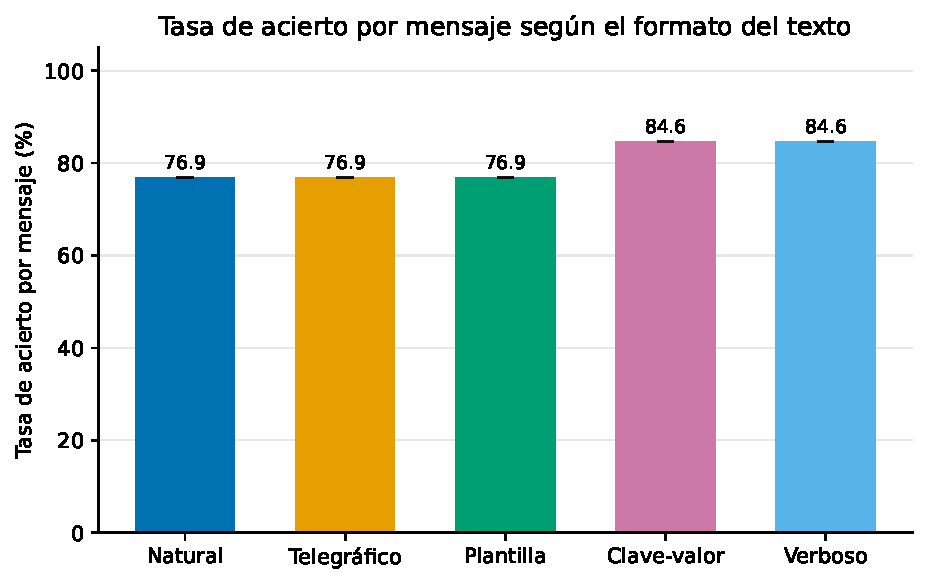
\includegraphics[width=0.7\textwidth]{Imagenes/Vectorial/formatos_fig1_acierto_mensaje}
\end{center}
\caption{Tasa de acierto por mensaje según el formato (media de 3 repeticiones, desviación cero).}
\label{fig:anexoFormatosAcierto}
\end{figure}

\begin{figure}[htbp]
\begin{center}
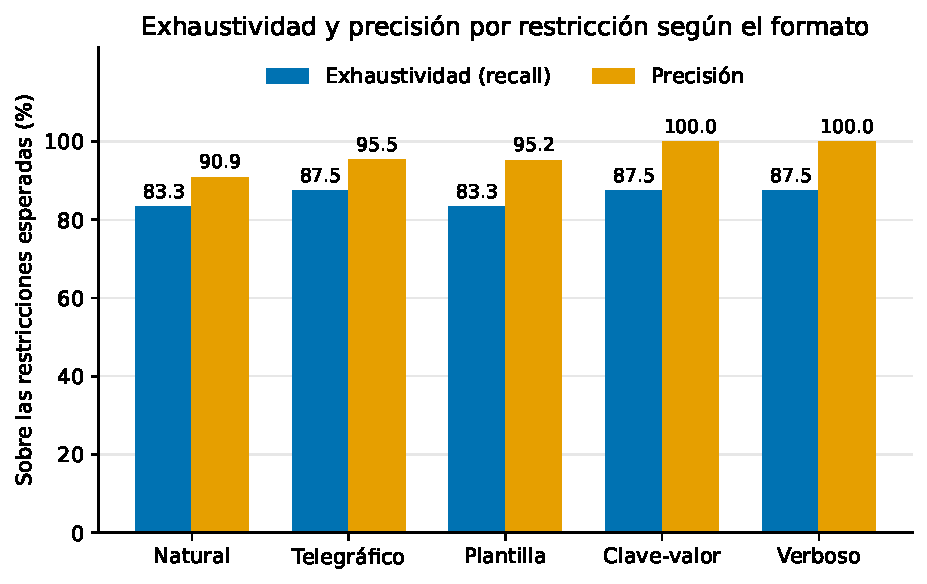
\includegraphics[width=0.85\textwidth]{Imagenes/Vectorial/formatos_fig2_recall_precision}
\end{center}
\caption{Exhaustividad y precisión por restricción, por formato.}
\label{fig:anexoFormatosRecall}
\end{figure}

\begin{figure}[htbp]
\begin{center}
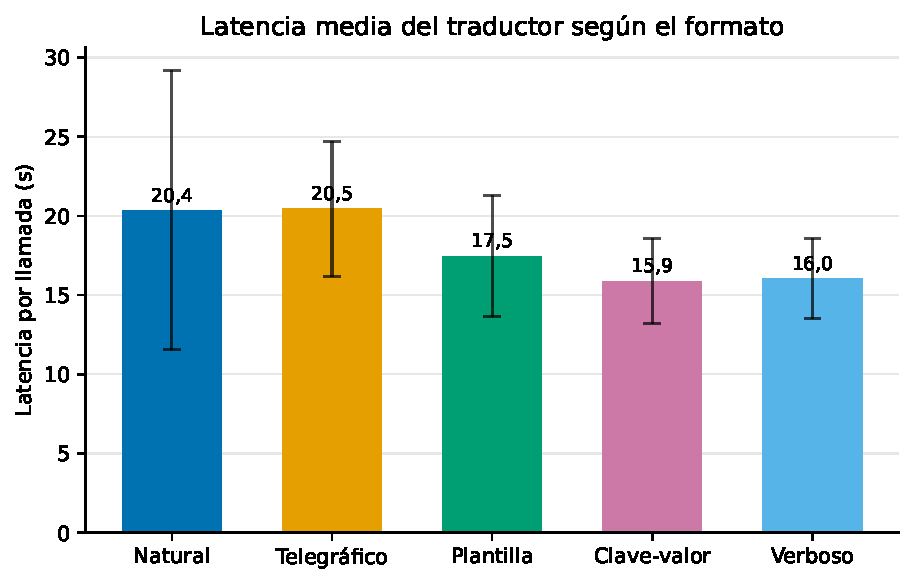
\includegraphics[width=0.7\textwidth]{Imagenes/Vectorial/formatos_fig3_latencia}
\end{center}
\caption{Latencia por llamada al traductor, por formato.}
\label{fig:anexoFormatosLatencia}
\end{figure}

\begin{figure}[htbp]
\begin{center}
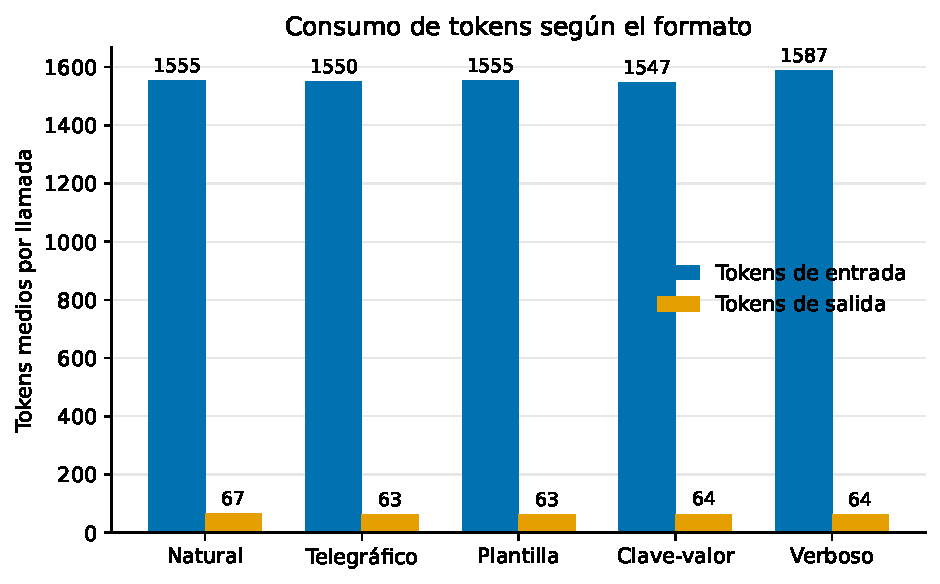
\includegraphics[width=0.7\textwidth]{Imagenes/Vectorial/formatos_fig4_tokens}
\end{center}
\caption{Tokens de entrada y salida por llamada, por formato.}
\label{fig:anexoFormatosTokens}
\end{figure}
